\section{Assessing Risk Preferences: A Dual-Criterion Approach}
\subsection{Setup and Definitions}
The results of section \ref{return_section} paint very different pictures of retail investors. 
Using the method set forth by \cite{Welch2022} and \cite{Fedyk2024}, analyzed also in section \ref{fedyk_paper_returns}, yields superior returns and similar drawdowns to the market.
They also conclude that the Robinhood crowd has achieved positive alpha when analyzed under different factor models (table VII, IX, X in \cite{Welch2022} and table 16 in \cite{Fedyk2024}). 
These results appear to be in contrast with the existing literature on retail investing, most notably \cite{BarberOdean2000}.

A more fundamental question, however, is whether those returns are attractive once investors' attitudes toward risk are taken into account.
This section evaluates the Robinhood portfolio against its market benchmarks using two complementary criteria.

First, I adopt the constant-relative-risk-aversion (CRRA) framework, in line with the majority of asset pricing work.
\begin{equation}
    U(W) = 
    \begin{cases}
    \frac{W^{1-\gamma}-1}{1-\gamma}, \gamma\neq 1\\
    \ln(W), \gamma = 1
    \end{cases}
    \label{CRRA}
\end{equation}

By computing the expected utility of both the Robinhood and benchmark portfolios over a grid of possible risk aversion ($\gamma$) values,
I identify the cutoff $\gamma^*$ such that a representative CRRA investor is indifferent between the two.
This delivers a concise, parametric summary of how risk preferences may shape portfolio choice.

Then, I estimate the welfare loss derived from investing in the Robinhood portfolio rather than (i)  not investing or (ii) investing in the market portfolio.
By comparing the certainty-equivalent wealth under each strategy for a CRRA investor, with risk aversion calibrated inside a feasible range,
I obtain dollar-denominated welfare losses that capture the risk-return profile taken by Robinhood investors.

However, this method cannot deliver precise estimates given the limited sample size. 
I therefore employ another method to estimate the risk aversion $\gamma$ from the percentage of wealth invested in the risky asset ($\alpha$), 
precise numbers about the wealth of Robinhood investors are not available, I therefore plot the implied risk aversion over a grid $\alpha$ and compare it to alternative portfolios.

\subsection{Expected Utility and Cutoff}
\subsubsection{Sampling Variability and Finite-Sample Limitations}
Identifying a cutoff level of risk aversion provides a clear criterion for the CRRA utility-maximizing investor: 
it is the minimum $\gamma$ at which an alternative strategy becomes preferred to the Robinhood portfolio.
However, the limited size and noise of the sample imply wide conference intervals for the estimated expected utilities at different $\gamma$ levels.
In practice, this remains a useful conceptual framework to understand how risk preference and beliefs may affect portfolio choice, but in limited samples, its numerical outputs are more illustrative than definitive.
However, this method yields precise results in a very specific case I will describe later. 

Formally, we want to find $\gamma^*$ defined as:
\begin{equation}
    \gamma^* = \min\left\{ \gamma_j : \mathbb{E}[U_p(\gamma_j)] \leq \mathbb{E}[U_m(\gamma_j)] \right\}
    \label{gamma_cutoff}
\end{equation}
where $U_p(\cdot)$ is the utility of the Robinhood portfolio, while $U_m(\cdot)$ is the utility of the market portfolio.

In practice, we apply CRRA utility function (\ref{CRRA}) to each gross return observation and then takes the sample average.
The resulting mean serves as the expected utility implied by the investor's revealed choices over the sample period.
Wealth at time $t$ is equal to gross returns, assuming the initial wealth $W$ to be equal to one without loss of generality.


The main problem related to this approach is inherent to the sample we apply it to, having only 539 observations and inclusion of extreme events such as the COVID crash. 
These factors inflate the sample variability of our mean-utility estimates, so much that regardless of whether we use daily returns, various rolling-window horizons, or subperiods, the resulting confidence intervals remain prohibitively wide.
Figure \ref{fig:cutoff} illustrates this well: 
\begin{figure}[H]
    \centering
    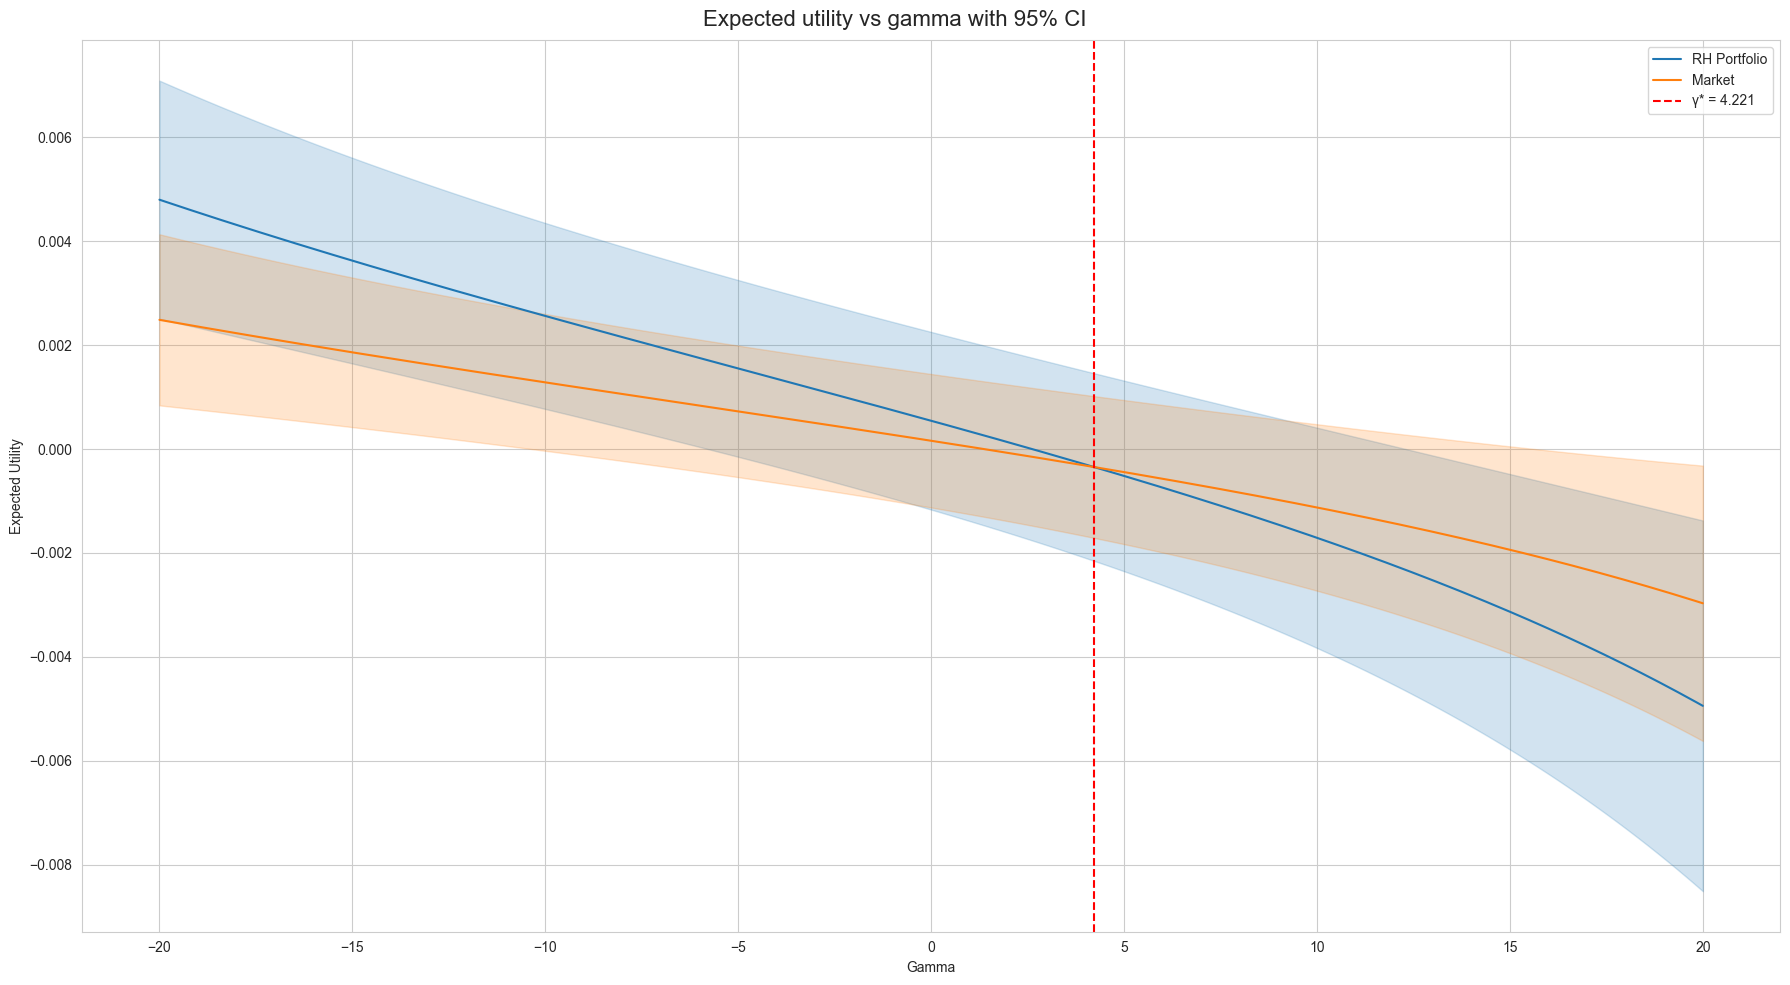
\includegraphics[width=\linewidth]{../images/risk/cutoff_daily.png}
    \caption{Utility for the Robinhood and Market portfolios evaluated over a grid of $\gamma$.}
    \label{fig:cutoff}
\end{figure}

\subsubsection{Augmented Return Sample via All Date-Pairs}
\label{sec:allpairs}
To overcome the limited information in only 539 daily observations, we construct an "all-pairs" dataset that dramatically amplifies our effective sample.  
Specifically, let the trading-day indices in our original series be $1,2,\dots,T$.  
For every ordered pair of dates $(i,j)$ with $1 \le i < j \le T$, we compute the cumulative excess return (net of the risk-free rate) between day $i$ and day $j$ as
\begin{equation}
    R_{i,j}
    \;=\;
    \prod_{k=i+1}^{j}\bigl(1 + r_k - r_{f,k}\bigr),
    \quad
    1 \le i < j \le T,
    \label{eq:allpairs_return}
\end{equation}
where $r_k$ is the portfolio return on day $k$ and $r_{f,k}$ is the daily risk-free rate.  
Using excess returns over the risk-free rate is necessary due to the changes in macroeconomic policy during the time of the sample. 
We treat each multi-day return $R_{i,j}$ as a separate outcome in the investor's distribution of possible holding-period returns, we increase the number of observations from $T$ to $T(T-1)/2$, which reduces sampling variability in our utility-based estimates.  
This "all-pairs" approach preserves the time-ordering of returns while allowing us to evaluate expected utility cutoffs with far greater precision.  

In practice, this results in finding a very low $\gamma^*$ that satisfies equation \ref{gamma_cutoff}, meaning that every investor with a reasonable risk-aversion parameter under CRRA utility would have a greater utility by investing in the market\footnote{
Both the risk-free rate and market returns are downloaded from Kenneth R. French data library \url{https://mba.tuck.dartmouth.edu/pages/faculty/ken.french/data_library.html}}.
In some cases, particularly when ending the sample before the pandemic, the utility curves fitted on the "all-pairs" dataset simply do not intersect for a wide grid of possible risk aversion,
and in fact we find also that in these cases the market stochastically dominates the robinhood portfolio (something which will be analyzed more in depth later).

Performing this exercise for the whole period on the two alternative Robinhood portfolios yields very telling results.
In both instances the cutoff risk aversion as defined in \ref{gamma_cutoff} is negative; 
in particular, the portfolio I constructed has a cutoff risk aversion of -5.437 while the one built using the alternative method we obtain -5.239.
The plot below shows this finding, only extremely risk loving investors would prefer the Robinhood portfolios over a diversified index.  

\begin{figure}[H]
  \centering
  \subfloat[Robinhood Returns Built from Prices]{%
    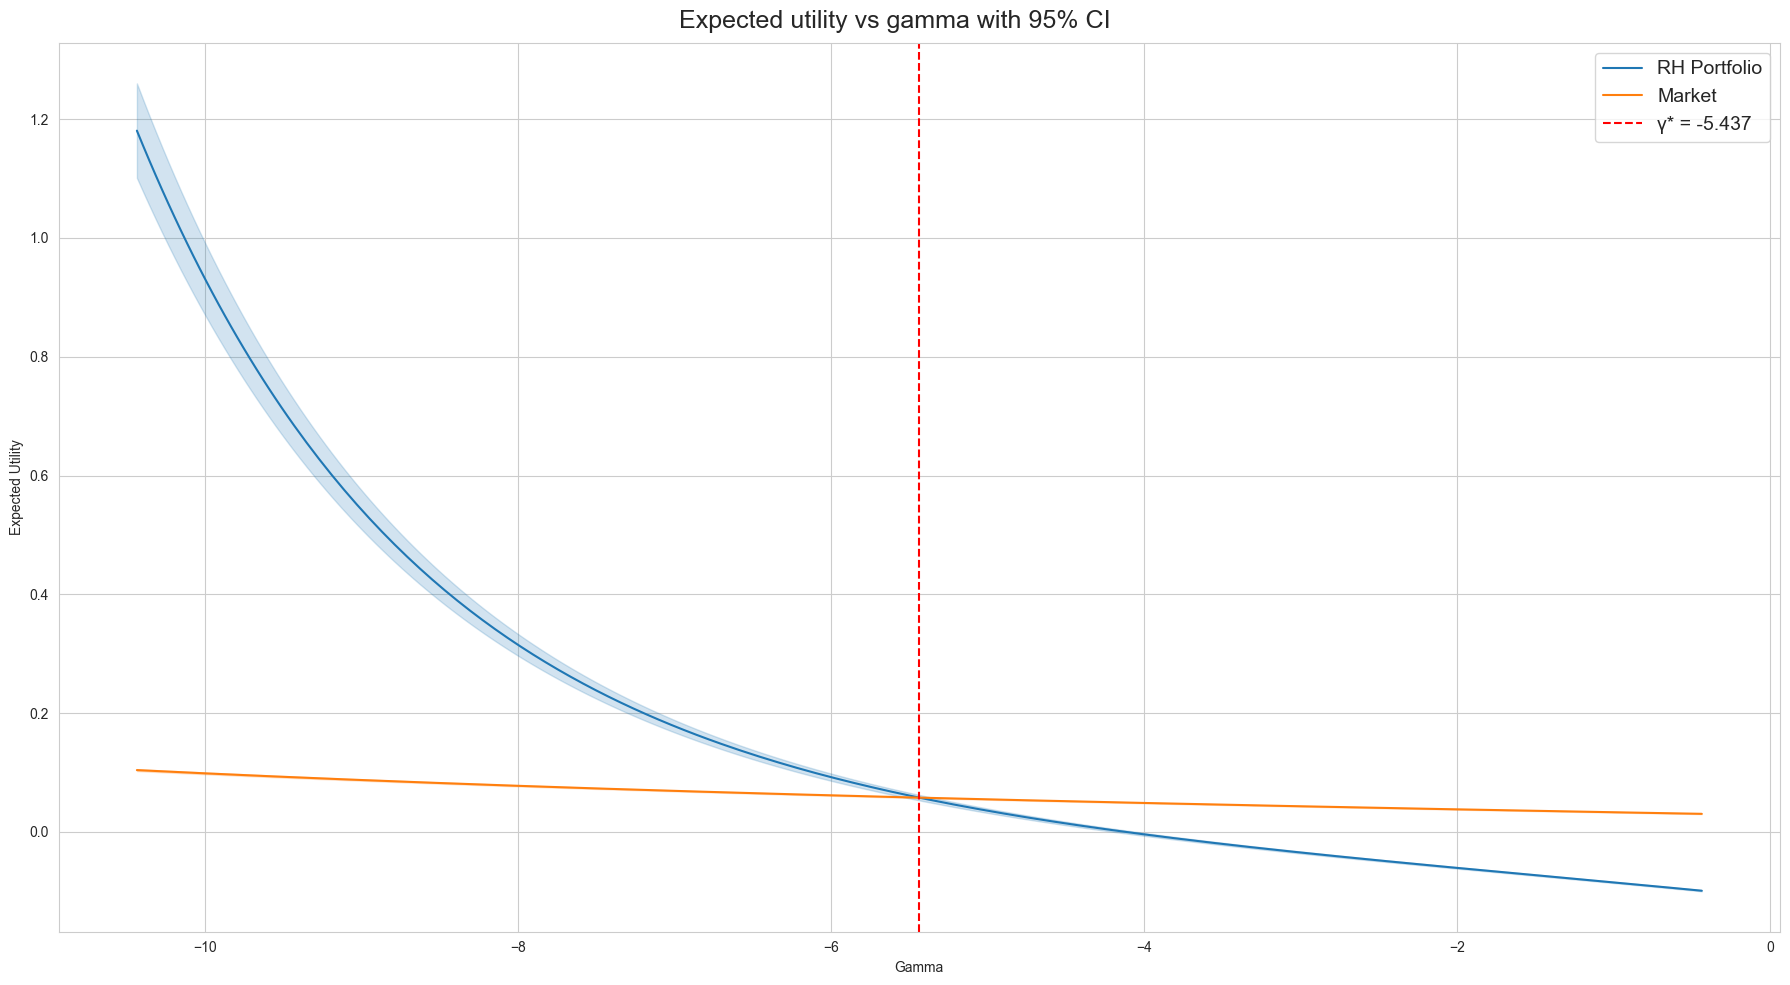
\includegraphics[width=0.48\textwidth]{../images/risk/cutoff_number_all.png}%
    \label{fig:cutoff_number_all}
  }
  \hfill
  \subfloat[Robinhood Returns Built Following Fedyk]{%
    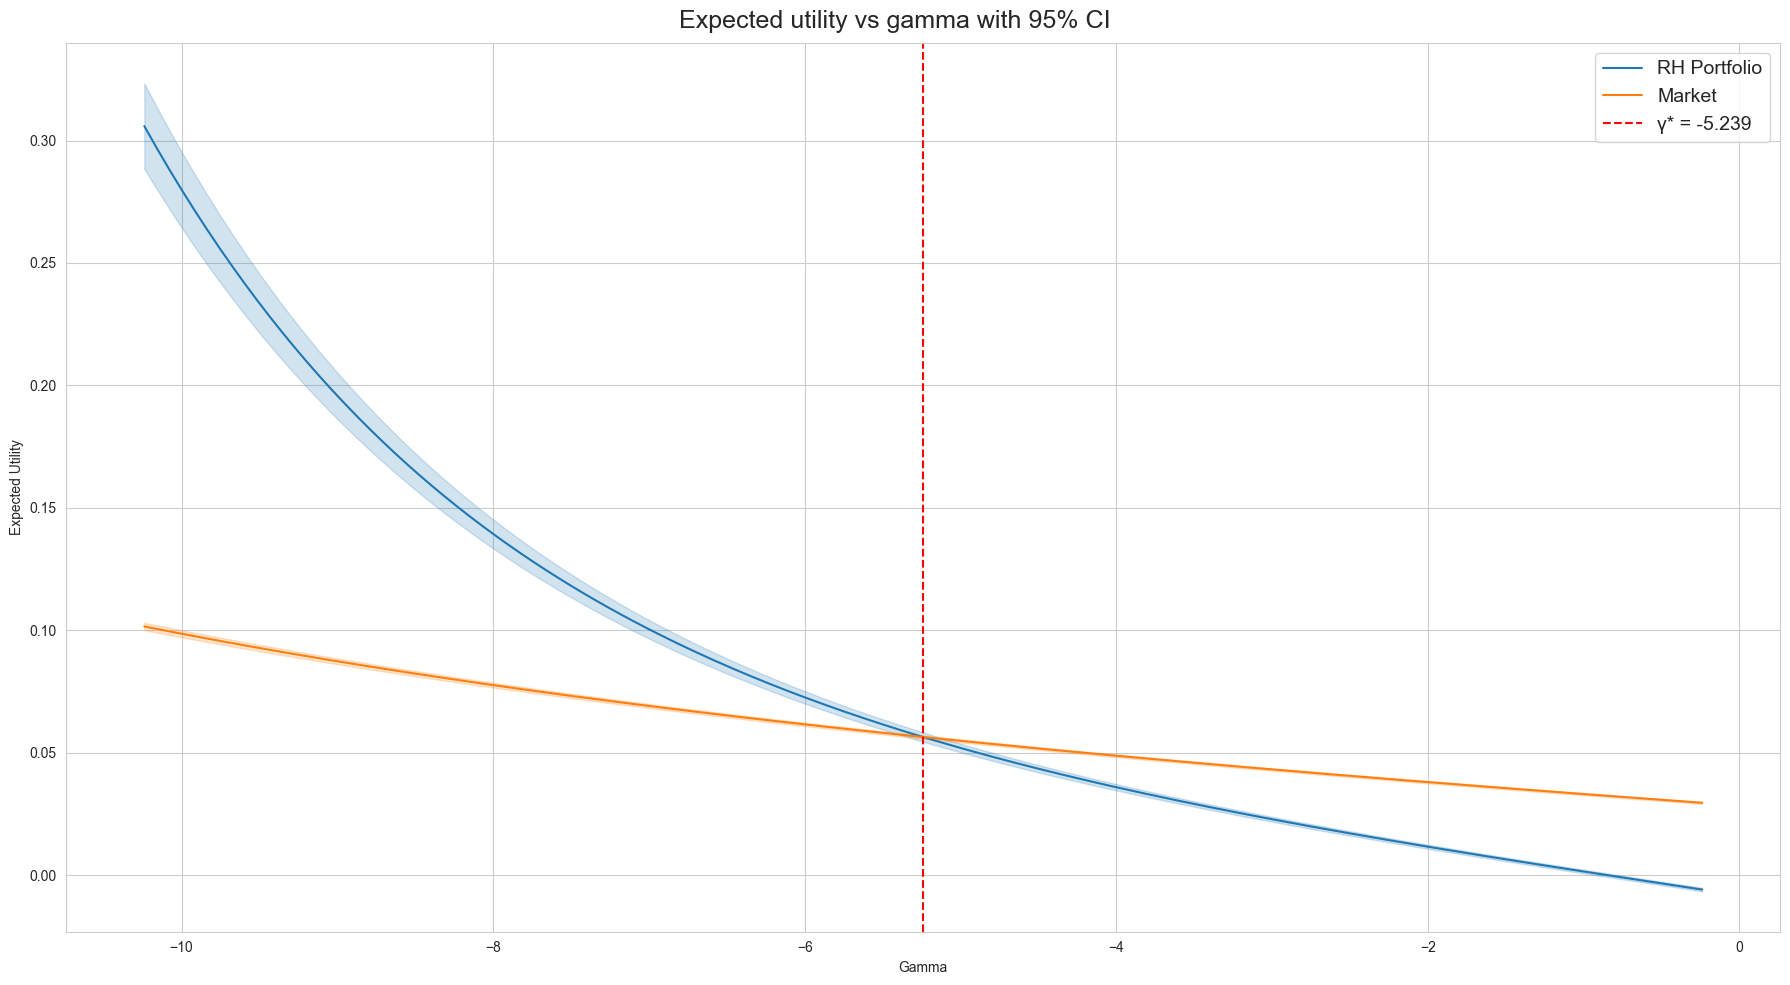
\includegraphics[width=0.48\textwidth]{../images/risk/cutoff_wealth_all.png}%
    \label{fig:cutoff_wealth_all}
  }
  \caption{Expected Utility and Cutoff Risk-aversion for the Robinhood and Market Portfolio.}
  \label{fig:cutoff_all_sidebyside}
\end{figure}

The only case in which $\gamma^*$ is positive is when we compare the Fedyk Portfolio and the World equity ETF as a proxy for the market index, obtaining a value of 1.214.
This implies that weakly risk-averse and risk-loving investors would have a greater utility by investing in this index.
However, if we limit the analysis to the pre-COVID period, the utility of the World ETF strictly dominates for each $\gamma\geq-15.813$, 
highlighting that the former result might indeed be a result of the volatility experienced in early 2020.  

\subsection{Implied Risk Aversion Approach}
\subsubsection{Deriving the Condition}
To address the limitations of our cutoff $\gamma$ approach, we turn to the canonical condition of maximizing expected utility by changing the share of wealth invested in the risky asset.  
In this framework, the agent decides to invest an amount $\alpha$ in the risky asset, his final wealth is therefore:
\begin{equation}
    W_1 = (1-\alpha) W_0 R_f  + \alpha W_0 \tilde R 
    \label{risky_portfolio}
\end{equation}
where $W_0$ is the initial wealth, which we can assume w.l.o.g equal to 1, $R_f$ is the gross return of the risk free asset and $\tilde R$ is the random variable that expresses the returns in the risky asset.

Defining $r=\tilde R - R_f$ we can approximate the CRRA utility of \ref{risky_portfolio} with a second-order taylor expansion around $R_f$:
\begin{equation}
    \mathbb{E}[U(W_1)] \approx R_f^{-\gamma} [\alpha \mathbb{E}[r] - \frac{\gamma}{2}\alpha^2\mathbb{E}[r^2]]
\end{equation} 

The investor chooses its portfolio to maximize the expected utility:
\begin{equation}
    \max_{0 \,\le\, \alpha \,\le\, 1}\; \mathbb{E}[U(W_1)]
    \;\approx\;
    \max_{0 \,\le\, \alpha \,\le\, 1}\;
    R_f^{-\gamma}\Bigl[\alpha\,\mathbb{E}[r]\;-\;\tfrac{\gamma}{2}\,\alpha^2\,\mathbb{E}[r^2]\Bigr]
\end{equation}

which yields the following equation\footnote{
    Derivation:
    $\text{FOC:}\quad
    \frac{\partial}{\partial \alpha}\Bigl\{R_f^{-\gamma}[\alpha\,\mathbb{E}[r]-\tfrac{\gamma}{2}\alpha^2\mathbb{E}[r^2]]\Bigr\}
    =
    R_f^{-\gamma}\bigl(\mathbb{E}[r]-\gamma\,\alpha\,\mathbb{E}[r^2]\bigr)
    \;=\;0$}:
\begin{equation}
    \alpha^*=
    \frac{\mathbb{E}[r]}{\gamma\,\mathbb{E}[r^2]}
\end{equation}

where $\mathbb{E}[r]=\mu-R_f$ and $\mathbb{E}[r^2]=\sigma^2+(\mu-R_f)^2$. 
Since returns are small, $(\mu-R_f)^2\ll\sigma^2$. We derive the following:
\begin{equation}
    \gamma^* = \frac{\mu-R_f}{\alpha \sigma^2}
    \label{gamma_star}
\end{equation}

In our case, both $\alpha$ and $\gamma$ are unknown. 
The variable of interest is $\gamma$, we can therefore use \ref{gamma_star} to compute it for every $\alpha$ in $[0,1]$. 


\subsubsection{Empirical Estimates and Interpretation}
\label{sec:gamma_estimates}
Since we have limited $\alpha$ to be in $[0,1]$ and $\sigma^2 \geq 0$, the implied risk aversion can be negative only if the mean excess returns are negative.

Another relevant point that should be discussed is the choice of not using rolling returns. 
Although they provide a good proxy for assessing the typical return over different horizons and across secruties, 
these return series suffer from autocorellation by construction, implying a very small variance especially at longer horizons.
Therefore, the risk aversion estimates provided by \ref{gamma_star} are unreliable and orders of magnitude greater than acceptable values in asset pricing.
For this reason, we focus or attention on daily, weekly, monthly and bi-monthly returns starting from the first day in the sample. This will avoid the problem with autocorrelation and provide interpretable and useful estimates over different horizons.


In table \ref{tab:gamma_implied} we report the implied share invested in the risky asset given a feasible upper and lower bound for investor's risk aversion, namely $\gamma=2$ and $\gamma=5$,
across all horizons.
As expected, $\alpha$ falls in a hyperbolic fashion, since \ref{gamma_star} implies $\alpha \propto \frac{1}{\gamma}$.

Across all four holding-period horizons and securities, lower risk aversion implies substantially higher optimal equity weights ($\alpha^*$) tha higher risk aversion.
Comparing across strategies, the S\&P 500 series has the largest implied shares at $\gamma=2$, rising from 0.766 at one day to 0.890 at five days before settling at 0.708 by sixty days, while its $\gamma=5$ allocations remain above both Robinhood strategies throughout. 
The World ETF's position at the bottom of the table highlights its lower excess-return profile: even at the longest horizon its $\gamma=2$ weight of 0.328 barely matches the $\gamma=5$ allocation to the Robinhood portfolios. 
Between the two Robinhood constructions, Fedyk is uniformly more aggressive than Mine, its $\gamma=2$ allocations exceed Mine's by roughly 10-25 percentage points at every horizon, reflecting Fedyk's higher expected excess return per unit variance.